\subsection{Inyectividad y Epiyectividad}
Una función $f(x)$ es \textit{inyectiva} cuando,
$\forall a,b \in X, \;\; f(a)=f(b) \Rightarrow a=b$
, es decir cuando nunca mapea elementos distintos de su \textit{Dominio} a un mismo elemento del \textit{Codominio}.

Análogamente, se dice que una función f(x) es \textit{sobreyectiva}, o epiyectiva cuando, $\forall y \in Y, \, \exists x \in X, \;\; f(x)=y$, es decir, que para cada elemento $y$ en el codominio $Y$, hay al menos un elemento $x$ en el dominio $X$ de forma que $f(x) = y$.\\
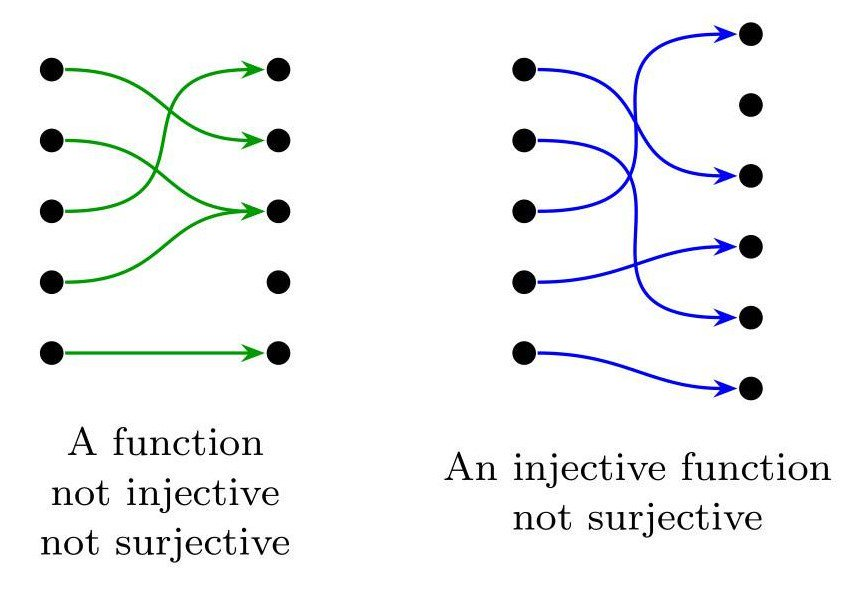
\includegraphics[width=\columnwidth]{inyectividad}\\
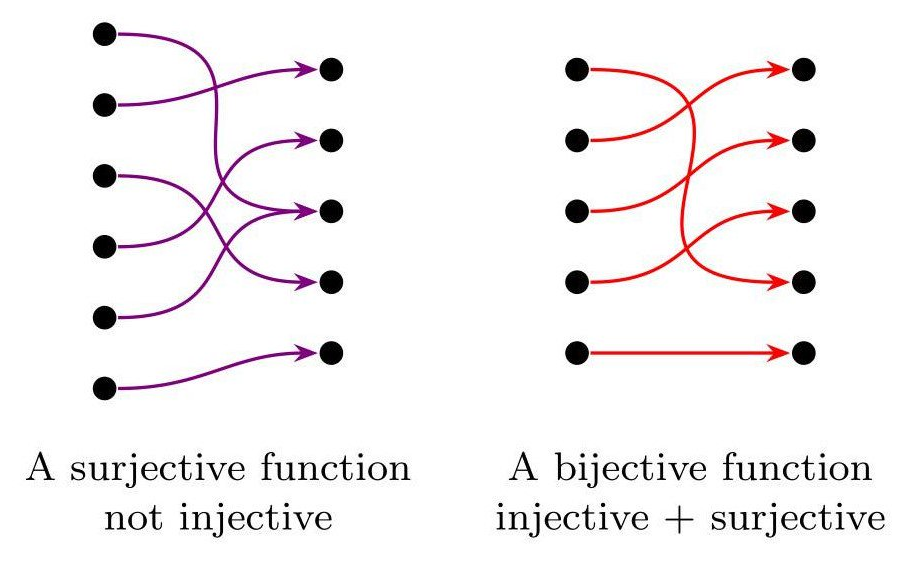
\includegraphics[width=\columnwidth]{sobreyectividad}